\section{Systematic Uncertainties}
\label{sec:uncertainties}

% In \Cref{sec:experimental_uncertainties}
%
% - Detector related uncertainties
% - Uncertainties related to the data-driven background estimates

% In \Cref{sec:theory_uncertainties}
% - Cross section uncertainties
% - Relative acceptance uncertainties
% - Acceptance uncertainties

% Uncertainties are tightly connected to the fit model thus here only
% give the 'definitions' of the uncertainties

% Additional post-processing (smoothing and pruning) steps will be
% described with the fit model in~\Cref{sec:}.

% The correlation scheme between uncertainties is further discussed
% with the fit model.

\subsection{Experimental Uncertainties}
\label{sec:experimental_uncertainties}

\begin{description}
\item[Integrated luminosity and pile-up] The integrated luminosity of
  the $pp$ collision dataset collected with the ATLAS detector in the
  period from 2015 to 2018 (\SI{139}{\per\femto\barn}) is measured
  with an uncertainty of
  \SI{1.7}{\percent}~\cite{ATLAS-CONF-2019-021}. This uncertainty is
  assigned to all processes estimated using simulation that are
  normalised using theoretical cross section. Additionally, an
  uncertainty on the reweighting of the instantaneous luminosity
  distribution used for the pile-up overlay in simulation to match the
  conditions of the $pp$ dataset is assigned to all simulated
  processes.

\item[Electrons] Uncertainties on electrons in simulation are obtained
  from dedicated calibration
  measurements~\cite{EGAM-2018-01,TRIG-2018-05} updated for the
  \SI{139}{\per\femto\barn} Run~2 dataset. The electron energy scale
  and resolution is measured in $Z \to e^+e^-$ events and propagated
  to predictions by shifting and smearing momenta of electrons in
  simulation. Uncertainties on the calibration of electron
  reconstruction, identification, isolation, and trigger efficiencies
  in simulation are obtained from measurements in~$J/\psi \to e^+e^-$
  and $Z \to e^+e^-$ events and applied as alternative weights to
  electrons in simulation.

  $e$-Veto efficiency.

\item[Muons]
  Muons... \cite{MUON-2018-03} \\
  Scale, (Sagitta) , (ID? MS?) \\
  Efficiencies: Reconstruction, Isolation, Trigger

\item[Taus]
  Taus... \\
  Scale \\
  Efficiencies: Reconstruction, Identification, eVeto (taus and
  electrons reconstructed as taus), Trigger

\item[Jets] Jets... (JVT, JES, JER) -- JES/JER \cite{JETM-2018-05}

\item[\pTmissAbs] MET

\item[Flavour tagging] Flavour tagging... \cite{FTAG-2018-01}

\end{description}

\begin{table}[htbp]
  \centering

  \caption{Table of CP uncertainties}%
  \label{tab:experimental_uncertainties}

  \begin{tabular}{lS[table-format=2]}
  \toprule
  Uncertainty source & {Components} \\
  \midrule
  Integrated luminosity & 1 \\
  Pile-up reweighting & 1 \\[0.5em]
  \textbf{Electrons} & \\
  Energy scale \& resolution & 3 \\
  Efficiencies (Reco., ID, Isol., Trigger) & 4 \\
  \tauhadvis $e^\pm$-veto efficiency & 2 \\[0.5em]
  \textbf{Muons} & \\
  Energy scale, ... & 5 \\
  Efficiencies (Reco., Isol., TTVA, Trigger) & 10 \\[0.5em]
  \textbf{Taus} & \\
  Energy scale & 4 \\
  Efficiencies (Reco., ID, $e$-Veto, Trigger) & 32 \\[0.5em]
  \textbf{Jets} & \\
  Energy scale & 33 \\
  Energy resolution & 14 \\
  Efficiency (jet vertex tagger) & 1 \\[0.5em]
  \textbf{Flavour tagging} & \\
  Efficiences (tag and mis-tag) & 13 \\[0.5em]
  \textbf{\pTmiss} & \\
  Momentum scale \& resolution & 3 \\
  \bottomrule
\end{tabular}

%%% Local Variables:
%%% mode: latex
%%% TeX-master: "../phd_thesis"
%%% End:

\end{table}

\todo[inline]{Where applicable, dedicated calibrations for ATLAS fast
  simulation are used.}

\todo[inline]{Experimental: MET -- all momentum / energy uncertainties are
  propagated to MET, additionally uncertainties related to the soft term}


\subsection{Theory uncertainties}%
\label{sec:modelling_uncertainties}%
\label{sec:theory_uncertainties}

A number of theoretical uncertainties have to be considered for signal
and background processes estimated using simulation. For a given
process these uncertainties are split, where applicable, into
uncertainties on the cross section of the process, uncertainties on
the acceptance of an analysis selection (e.g.\ the signal region
selection), and uncertainties affecting the acceptance in terms of the
shape of discriminants used for the statistical analysis. With few
exceptions, acceptance uncertainties on a given process that originate
from the same source are assumed to be fully correlated between all
analysis regions.

The description of theory uncertainties is divided into three parts.
First, the treatment of uncertainties on the major \ZHF and \ttbar
backgrounds is described, representing a special case since the cross
section of these processes is determined from the likelihood fit to
observed data. Subsequently, uncertainties on other background
processes estimated with simulation and normalised using theoretical
predictions are briefly outlined. Finally, uncertainties on the
modelling of the SM \HH and BSM $X \to \HH$ signals are presented.

%\subsubsection{Uncertainties on the relative acceptance of \ZHF and
% \ttbar between regions}
\subsubsection{Acceptance uncertainties on \ZHF and \ttbar backgrounds}

The normalisation of the \ZHF and \ttbar backgrounds are measured in
the combined likelihood fit of control and signal regions. Constraints
on the normalisation of the \ZHF background primarily originate from
the dedicated control region. The normalisation of the \ttbar
background is mainly constrained in the signal region of the \lephad
SLT channel and the \ZHF control region. Due to the determination of
the normalisation of these processes from the fit to data, any
uncertainties on their overall normalisation, for example
uncertainties on the total cross sections, are omitted. Uncertainties
changing the relative acceptance of \ZHF or \ttbar events between
regions have to be considered instead. These uncertainties will be
referred to as \emph{relative acceptance uncertainties},
hereafter. The approach outlined in the following was originally
adopted by the previously published analysis in this
channel~\cite{HIGG-2016-16-witherratum} from searches and measurements
of $VH$~($H\to\bbbar$)
production~\cite{HIGG-2016-29,HIGG-2018-04,HIGG-2018-51}.

Assuming a general case of a background process that is estimated
using simulation and normalised by a fit to data in two analysis
regions A and B, with region A being defined as the reference
region. In this case, the probability of an event to be selected in a
given region~R is given by the product of acceptance and efficiency,
$(\AccTimesEff)_{\text{R}}$, for this region. The simulation predicts
how \AccTimesEff relates between both regions and one can define the
ratio
\begin{align*}
  \mathcal{R} = \frac{(\AccTimesEff)_{\text{B}}}{(\AccTimesEff)_{\text{A}}} \,\text{,}
\end{align*}
which will be be referred to as the \emph{relative acceptance} between
regions A and B. Uncertainties on the modelling of $\mathcal{R}$ in
simulation are assigned as uncertainties on the normalisation of the
background process in region B\todo{Show mathematically?} and no
additional uncertainties are assigned in the reference region, A. They
are estimated by performing variations of the background prediction,
for example using alternative generator configurations, and estimating
a relative change of~$\mathcal{R}$ according to
\begin{align}
  \frac{\Delta \mathcal{R}}{\mathcal{R}} = \frac{\mathcal{R}(\text{variation}) - \mathcal{R}(\text{nominal})}{\mathcal{R}(\text{nominal})} \,\text{.}
  \label{eq:relative_acceptance_uncertainty}
\end{align}
The use of the relative acceptance for the definition of the modelling
uncertainties leads to a cancellation of variations that lead to the
same relative change in \AccTimesEff in both regions, which
corresponds to an overall change in normalisation that can be absorbed
into the freely floating normalisation factor.

% This uncertainty on the relative acceptance between the the
% reference region A and region B is included in the background model
% by assigning a normalisation uncertainty of
% $\Delta \mathcal{R} / \mathcal{R}$ on the background in region B.

% The absolute value\footnote{When introducing multiple regions, the
% relative sign of $\Delta \mathcal{R} / \mathcal{R}$ when comparing
% different regions to the same reference is important when
% correlating these uncertainties in the statistical analysis and is
% kept to allow to consistently define the variations.} of
% $\Delta \mathcal{R} / \mathcal{R}$ is considered the extrapolation
% uncertainty.

% The shape effects of uncertainties are estimated separately and will be described in~\Cref{sec:modelling_uncertainties}.

% Note: Sign is important -> direction of effect when correlating systematics

The relative acceptance uncertainties are defined using the \ZHF
control region as a reference region, providing constraints on both
the \ZHF and \ttbar backgrounds. The uncertainties are estimated
separately for the \ZHF and \ttbar backgrounds in the signal regions
(\hadhad, \lephad SLT, \lephad LTT). Uncertainties originating from
the same source are assumed to be fully correlated between all
analysis regions.

The relative acceptance uncertainties originating from the modelling
of the \ZHF background in simulation are estimated by performing
variations of the event generation process. A brief description of the
variations is given in the following, reproducing the prescriptions
developed by the ATLAS collaboration:
\begin{description}

\item[Factorisation and renormalisation scales] Six variations of the
  factorisation and renormalisation scales are performed using
  internal reweighting implemented in
  \SHERPA[2.2.1]~\cite{Bothmann:2019yzt}, altering the scales by
  factors of $\frac{1}{2}$ and $2$. The following variations are
  considered:
  \begin{align*}
    \left( \frac{\muF}{\muF^{\text{nom.}}}, \frac{\muR}{\muR^{\text{nom.}}} \right) \in
    \left\{ (\tfrac{1}{2}, \tfrac{1}{2}), (\tfrac{1}{2}, 1), (1, \tfrac{1}{2}), (1, 2), (2, 1), (2, 2) \right\} \,\text{,}
  \end{align*}
  where $\muF^{\text{nom.}}$ and $\muR^{\text{nom.}}$ are the nominal
  values of the scales.

\item[Resummation scale] The scale of the resummation of soft gluon
  emissions in the \SHERPA parton shower is varied by factors of
  $\frac{1}{2}$ and 2. Variations of the resummation scale are
  provided in parametrised form with respect to the default \SHERPA
  configuration in Ref.~\cite{anders:2017}.

\item[Multi-jet merging scale] The simulation of \Zjets events with
  \SHERPA[2.2.1] uses matrix elements of NLO accuracy for up to two
  and LO for up to four partons. These multi-parton matrix elements
  are merged with the parton shower using an extension of the CKKW
  algorithm~\cite{Catani:2001cc,Hoeche:2009rj,Hoeche:2012yf}. The
  characteristic scale~$Q_{\text{cut}}$ of the multi-jet merging
  algorithm is varied from its nominal value of
  $Q_{\text{cut}} = \SI{20}{\GeV}$ to \SI{15}{\GeV} and
  \SI{30}{\GeV}~\cite{anders:2017}. These variations are provided,
  following the approach for the resummation scale, in parametrised
  form in Ref.~\cite{anders:2017}.
  %\cite{ATLAS:2021yza}

\item[PDF+\alphas and PDF choice] Uncertainties on the \NNPDF[3.0nnlo]
  set of PDFs~\cite{Ball:2014uwa} are evaluated using 100 replica sets
  provided through the \textsc{LHAPDF6} library~\cite{Buckley:2014ana}
  and implemented using internal reweighting in \SHERPA. The
  uncertainty on \alphas propagated by comparing \NNPDF[3.0nnlo] PDF
  sets with $\alphas(\mZ^2) = 0.117$ and $0.119$ with the nominal set
  using a value of $0.118$. Finally, an uncertainty on the choice of
  PDF set is estimated by comparing with two alternative PDF sets
  \MMHT[nnlo68cl]~\cite{Harland-Lang:2014zoa} and
  \CT[14nnlo]~\cite{Dulat:2015mca}.

\item[Alternative generator and parton shower] The prediction of
  \Zjets with the default configuration of \SHERPA[2.2.1] is compared
  to an alternative setup using~\MGNLO[2.2.2]~\cite{Alwall:2014hca}
  for the calculation of the hard interaction at LO interfaced
  to~\PYTHIA[8.186]~\cite{Sjostrand:2007gs} for parton showering.

\end{description}
Relative acceptance uncertainties on the \ZHF background are derived
using these variations according
to~\Cref{eq:relative_acceptance_uncertainty} for the three signal
regions. The uncertainties are summarised
in~\Cref{tab:uncertainties_zhf_extrapol} separately for all sources of
uncertainty.

The \lephad SLT signal region selection is the closest to the \ZHF
control region, resulting in a small relative acceptance uncertainty
of approximately \SI{9}{\percent}. The \hadhad and \lephad LTT
channels deviate yielding an uncertainty of approximately
\SI{16}{\percent}. In all cases the dominant sources of uncertainty
are the scale variations as well as the comparison with
\MGNLO+\PYTHIA[8]\todo{``Interpretation'' needs some work.}.

The relative acceptance uncertainties on the \ttbar background are
estimated using a similar approach. The prescriptions documented in
Ref.~\cite{ATL-PHYS-PUB-2020-023} are used to estimate modelling
uncertainties on the nominal prediction obtained from simulation with
\POWHEGBOX[v2]+\PYTHIA[8]. A revised version of these prescriptions
was previously presented in~\Cref{sec:bkg_hadhad_ttbarfakes} as part
of the \ttbarFakes scale factor measurement. In the following, the
prescriptions are summarsied, highlighting the differences with
respect to the previous description.

The uncertainty of the modelling of the hard interaction (parton
shower) is evaluated by replacing \POWHEGBOX[v2] (\PYTHIA[8]) with
\MGNLO (\HERWIG[7]) for the matrix element (parton shower)
generation. Explicit variations of the scales, and \PYTHIA[8] damping
parameter, $\hdamp$, are omitted. Instead they are included in the
variations of the initial-state radiation. The uncertainties on the
amount of final-state radiation and the PDF+\alphas uncertainties are
estimated using internal reweighting in \PYTHIA[8]. The relative
acceptance uncertainty for \ttbar backgrounds in the three signal
regions is given in~\Cref{tab:uncertainties_ttbar_extrapol}.

\begin{table}[htbp]
  \centering

  \caption{Relative acceptance uncertainties on the \ZHF (a) and
    \ttbar background (b) in the three signal regions. The relative
    sign of the effect of variations between the signal regions is
    indicated by the ``$\pm$'' and ``$\mp$'' prefixes. The total
    uncertainty is given for illustration of the size of the
    uncertainties only.}

  \begin{subtable}[t]{0.95\textwidth}
    \centering
    \subcaption{\ZHF ($Z+bb$, $Z+bc$, $Z+cc$) background}%
    \label{tab:uncertainties_zhf_extrapol}

    \begin{tabular}{lccc}
  \toprule
  & \multicolumn{3}{c}{Signal region} \\
  \cline{2-4}
  Uncertainty source & {\hadhad} & {\lephad SLT} & {\lephad LTT} \\
  \midrule
  \MGNLO+\PYTHIA[8] & $\pm 7.0\,\%$ & $\mp 2.1\,\%$ & $\mp 11\,\%$ \\[0.2em]
  Factorisation and renormalisation scale & $\substack{+12 \\ -9.7}\,\%$ & $\substack{+5.4 \\ -3.0}\,\%$ & $\substack{+8.5 \\ -3.0}\,\%$ \\[0.2em]
  Multi-jet merging (CKKW) & $\pm 5.4\,\%$ & $\pm 7.0\,\%$ & $\pm 7.2\,\%$ \\[0.2em]
  Parton shower resummation scale (QSF) & $\mp 6.0\,\%$ & $\pm 1.7\,\%$ & $\pm 1.6\,\%$ \\[0.2em]
  Alternative PDF sets & $\pm 1.0\,\%$ & $ \pm 1.0\,\%$ & $\pm 1.1\,\%$ \\[0.2em]
  PDF+\alphas (\NNPDF[3.0nnlo]) & $\pm 0.77\,\%$ & $\pm 0.27\,\%$ & $\pm 0.35\,\%$ \\
  \midrule
  Total & $\substack{+16\\-15}\,\%$ & $\substack{+9.3\\-8.1}\,\%$ & $\substack{+16\\-14}\,\%$ \\
  \bottomrule
\end{tabular}

%%% Local Variables:
%%% mode: latex
%%% TeX-master: "../phd_thesis"
%%% End:

  \end{subtable}

  \vspace{10pt}

  \begin{subtable}[t]{0.95\textwidth}
    \centering
    \subcaption{\ttbar background}%
    \label{tab:uncertainties_ttbar_extrapol}

    \begin{tabular}{lccc}
  \toprule
  & \multicolumn{3}{c}{Signal region} \\
  \cline{2-4}
  Uncertainty source & {\hadhad} & {\lephad SLT} & {\lephad LTT} \\
  \midrule
  ME & $\mp 3.8\,\%$ & $\mp 0.3\,\%$ & $\pm 0.9\,\%$ \\[0.2em]
  PS & $\pm 2.2\,\%$ & $\pm 7.2\,\%$ & $\pm 8.8\,\%$ \\[0.2em]
  ISR & $\mp 0.3\,\%$ & $\mp 0.9\,\%$ & $\pm 1.3\,\%$ \\[0.2em]
  FSR & $\substack{-4.5\\+2.0}\,\%$ & $\substack{-1.0\\+1.5}\,\%$ & $\substack{-3.2\\+1.0}\,\%$ \\[0.2em]
  PDF+\alphas & $\pm 0.2\,\%$ & $\pm 0.6\,\%$ & $\pm 0.8\,\%$ \\
  \midrule
  Total & $\substack{+4.8\\-6.3}\,\%$ & $\pm 7.4\,\%$ & $\substack{+9.0\\-9.4}\,\%$ \\
  \bottomrule
\end{tabular}

%%% Local Variables:
%%% mode: latex
%%% TeX-master: "../phd_thesis"
%%% End:

  \end{subtable}
\end{table}

Relative acceptance uncertainties are implemented as uncertainties on
the normalisation of the respective backgrounds in signal regions
only. Variations of the modelling in simulation can also change the
shapes of discriminants used for signal extraction, including $\mll$
in the \ZHF control region, which have to be considered.

The impact of modelling uncertainties on distributions of the MVA
discriminants in the signal regions and the \mll distribution in the
\ZHF control region are investigated by performing shape comparisons
of the varied and nominal distributions. In cases where the shapes do
not differ significantly, no additional uncertainties are assigned.
When deviations are observed, the shape uncertainties are propagated
to the discriminants and correlated with the corresponding
normalisation uncertainty.

Shape uncertainties on the \ZHF background are considered for the
comparison with the alternative event generation setup changing both
the matrix element and the parton shower generator (\hadhad), and for
variations of the factorisation and renormalisation scales (\hadhad,
\lephad SLT \& LTT). All other variations, including variations in the
\ZHF control region, are found to have negligible impact on the shape
of the discriminating variables (\mll / MVA scores).

Shape uncertainties on the \ttbar background are considered for the
comparison with alternative matrix element generator and parton shower
programs (\hadhad, \lephad SLT), and the uncertainty on the amount of
initial- and final-state radiation (\hadhad). All other variations
have negligible impact of the shapes of the relevant distributions.


\subsubsection{Uncertainties on minor backgrounds}

The minor backgrounds considered by the analysis are normalised using
cross sections from theory and thus both cross section as well as
acceptance uncertainties are considered. In contrast to the major
backgrounds, shape uncertainties on minor backgrounds are neglected
and only uncertainties on the normalisation are considered (with the
exception of the $tW$ acceptance uncertainties).  A brief description
of the uncertainties on minor backgrounds is given in the following:
\begin{description}

\item[$Z + (bl, cl, ll)$] A normalisation uncertainty of
  \SI{5}{\percent} is assigned to account for the uncertainty on the
  predicted cross section of \Zjets production at
  NNLO~\cite{Anastasiou:2003ds} used to normalise the
  sample. Additionally, an acceptance uncertainty of \SI{23}{\percent}
  is adopted from Ref.~\cite{HIGG-2018-51}.

\item[$W + \text{jets}$] A \SI{5}{\percent} cross section uncertainty
  is assigned to the NNLO cross section
  prediction~\cite{Anastasiou:2003ds}. A normalisation uncertainty of
  \SI{37}{\percent} is assigned in the \lephad channels adopted from
  Ref.~\cite{HIGG-2018-51}. This uncertainty is inflated to
  \SI{50}{\percent} in the \hadhad channel since the small \Wjets
  contribution is not part of the data-driven \faketauhadvis
  estimation.

\item[Diboson] Normalisation uncertainties of \SI{20}{\percent},
  \SI{26}{\percent}, and \SI{25}{\percent} are applied to $ZZ$, $WZ$,
  and $WW$ production, respectively. These uncertainties are adopted
  from Ref.~\cite{HIGG-2018-51}.

\item[Single top] Uncertainties on the cross section used to normalise
  the predictions are taken from Ref.~\cite{stopxsec}. A
  \SI{20}{\percent} acceptance uncertainty is assigned to the minor
  contribution of single top produced in $s$- and $t$-channel diagrams
  which is adopted from Ref.~\cite{HIGG-2018-51}.

  Acceptance uncertainties in the phase space selected by the analysis
  are derived for $tW$ production, which is the dominant source of
  single top background in this analysis. The acceptance uncertainties
  on the NLO+PS matching and the choice of parton shower program are
  estimated separately by comparison with alternative simulation
  setups using \MGNLO[2.6.2] and \HERWIG[7],
  respectively. Uncertainties on PDF+\alphas and the amount of
  initial- and final-state radiation are obtained by reweighting of
  the nominal simulation result. Finally, an uncertainty on the
  treatment of the removal of interference\todo{What happens to the
    interference? Neglected?  Included in \ttbar?} between $tW$ at NLO
  and \ttbar production is estimated by performing MC-to-MC
  comparisons of the nominal diagram removal and diagram subtraction
  schemes~\cite{Frixione:2008yi}.

  The total acceptance uncertainty on $tW$ production is
  \SI{34}{\percent}, \SI{14}{\percent}, \SI{23}{\percent} in the
  \hadhad, \lephad SLT, and \lephad LTT signal region,
  respectively. The shape effect of the FSR and $tW$-$\ttbar$
  interference uncertainties on the MVA discriminants are propagated
  using suitable parametrisations.

\item[Single SM $H$ production] Uncertainties on the total cross
  section of the SM $H$ production modes considered as backgrounds are
  assigned according to the recommendations in
  Ref.~\cite{deFlorian:2016spz} for $m_{H} =
  \SI{125.0}{\GeV}$. Analogously, uncertainties on the branching
  ratios of $\PHiggs \to \tautau$ and $\PHiggs \to \bbbar$ are
  assigned to the relevant processes and are taken from
  Ref.~\cite{deFlorian:2016spz}.

  An acceptance uncertainty of \SI{100}{\percent} is assigned to
  $H \to \tautau$ backgrounds produced via ggF, VBF, and $WH$ to
  account for difficulties in the modelling of produced in association
  with heavy flavour quarks\todo{Citation?} and the lack of a
  dedicated background estimate for single Higgs bosons production via
  $bbH$.

  Acceptance uncertainties in the phase space selected by the analysis
  are derived for single Higgs boson backgrounds produced via $ZH$,
  $\ttbar H$ for both $H \to \tautau$ and $H \to \bbbar$. They are
  derived by varying the parton shower program (\HERWIG[7]),
  PDF+\alphas, and factorisation / renormalisation scales and assigned
  as normalisation uncertainties when non-negligible. Additionally for
  $\ttbar H$ production, an uncertainty on the NLO+PS matching is
  assigned by comparing with an alternative generator
  (\MGNLO[v2.6.0]), and uncertainties targeting the modelling of
  initial- and final-state radiation.
\end{description}

\todo[inline]{No uncertainties on $ttW$ and $ttZ$?}

\begin{table}[htbp]
  \centering

  \missingfigure[figwidth=0.75\textwidth]{Summary of bkg uncertainties.}

  \caption{Summary of minor background uncertainties}
\end{table}

\subsubsection{Signal modelling uncertainties: SM $HH$}

% CROSS SECTION
Uncertainties on the cross section of the SM $HH$ production in the
ggF and VBF production modes are considered when the signal strength,
$\mu = \sigma / \sigma_{\text{SM}}$, is used as a parameter of
interest (POI). When the total SM $HH$ cross section is the POI, the
cross section uncertainties are omitted.

The uncertainty on the cross section of SM $HH$ in the ggF production
mode at NNLO~\FTapprox~\cite{Grazzini:2018bsd} consists of an
uncertainty on PDF+\alphas of \SI{\pm 3.0}{\percent}~\cite{LHCHWGHH}
and an uncertainty from scale variations and the scheme used for the
treatment of the mass of the virtual top in the heavy-quark loop of
$^{+6\%}_{-23\%}$~\cite{Baglio:2020wgt}. For the VBF production mode,
which is normalised using cross section at
N$^3$LO~\cite{Dreyer:2018qbw}, the scale uncertainties
are~$^{+0.03\,\%}_{-0.04\,\%}$~\cite{LHCHWGHH} and the uncertainty from
PDF and \alphas is~\SI{\pm 2.1}{\percent}~\cite{LHCHWGHH}.

Uncertainties on the branching ratios of $H \to \tautau$ and
$H \to \bbbar$ are taken from Ref.~\cite{deFlorian:2016spz} and
assigned as uncertainties on the signal normalisation.

Signal acceptance uncertainties are derived in all regions by
performing variations of the signal prediction.
% The variations are ensured to leave the total cross section
% invariant to prevent double-counting of cross section uncertainties.
The uncertainty on the choice of the parton shower program is
estimated by comparing the nominal signal generation using
\PYTHIA[8.244] for parton showering with an alternative using
\HERWIG[7.1.6]. An uncertainty from the effect of missing higher
orders in the pertubative expansion is estimated by performing six
variations of the factorisation and renormalisation scales using
internal reweighting of the generator. Uncertainties on the PDF sets
are estimated using the prescriptions for the
\PDFforLHC[15nlo]~\cite{Butterworth:2015oua} and
\NNPDF[3.0nlo]~\cite{Ball:2014uwa} PDF sets for ggF and VBF,
respecively. The PDF uncertainties are provided in the form of 30
eigenvariations for \PDFforLHC[15nlo] and 100 replica sets for
\NNPDF[3.0nlo]. Finally, the value of $\alphas(\mZ^2)$ is varied up
and down by 0.0015 (0.001) about the central value of $0.118$ in the
\PDFforLHC[15nlo] (\NNPDF[3.0nlo]) PDF set.

% The \PDF4LHC[15nlo] prescription uses 30
% eigenvariations of the PDF set that are independently propagated to
% the observables and the deviations from the nominal value are added in
% quadrature to yield the uncertainty. For \NNPDF[3.0nlo] PDF set which
% provides uncertainties in the form of MC replicas, the uncertainty is
% defined by the sample standard deviation of the observable determined
% using 100 replicas of the PDF set.

The acceptance uncertainties on the SM $HH$ signal are summarised
in~\Cref{tab:theory_uncertainty_signal} for the considered production
modes. The uncertainties on PDF+\alphas are found to be negligible in
most cases and thus omitted. The impact of the variations on the shape
of the MVA discriminants is found to be negligible in most cases. The
variations of the factorisation and renormalisation scales for the VBF
production mode in the \hadhad signal region is found to induce small
changes in the shape (up to \SI{2}{\percent} in bins sensitive to the
SM $HH$ signal) of the SM $HH$ BDT score distribution which is
implemented as a shape uncertainty for later statistical evaluation.

\begin{table}[htbp]
  \centering

  \caption{Theory uncertainties on the acceptance of non-resonant SM
    $HH$ signals in the three signal regions. Uncertainties marked as
    ``--'' are negligible.}%
  \label{tab:theory_uncertainty_signal}

  \begin{tabular}{l
  S[retain-explicit-plus]
  S[retain-explicit-plus]
  S[retain-explicit-plus]}
  \toprule
  & \multicolumn{3}{c}{Acceptance uncertainty / \%} \\
  \cmidrule{2-4}
  Source & {\hadhad} & {\lephad SLT} & {\lephad LTT} \\
  \midrule
  \multicolumn{4}{c}{SM $HH$ (ggF production mode)} \\
  \midrule
  Parton shower       & \pm 4.3 & \pm 7.6 & \pm 7.5 \\
  Scales (\muF, \muR) & \pm 1.4 & \pm 1.2 & \pm 1.0 \\
  PDF+\alphas & {--} & {--} & {--} \\
  \midrule
  \multicolumn{4}{c}{SM $HH$ (VBF production mode)} \\
  \midrule
  Parton shower & \pm 3.0 & \pm 6.3 & \pm 2.1 \\
  Scales (\muF, \muR) & {--$^\dagger$} & \pm 1.0 & \pm 1.0 \\
  PDF+\alphas & \pm 1.0 & {--} & {--} \\
  \bottomrule
\end{tabular}

%%% Local Variables:
%%% mode: latex
%%% TeX-master: "../phd_thesis"
%%% End:

\end{table}

\todo[inline]{Acceptance uncertainties are assumed to be fully
  correlated across channels but uncorrelated across production
  modes.}

\subsubsection{Signal modelling uncertainties: BSM $gg \to X \to HH$}

Cross section uncertainties are not considered for the production of
heavy scalar resonances in BSM scenarios since the cross
section~$\sigma(gg \to X \to HH)$ is used as the POI. However,
uncertainties on the SM Higgs boson branching ratios are considered
according to Ref.~\cite{deFlorian:2016spz}.

Acceptance uncertainties on BSM \HH production are estimated for the
choice of parton shower program, factorisation and renormalisation
scales, and PDF+\alphas. The uncertainties are calculated for a subset
of resonance masses considered in the analysis (due to the
availability of alternative samples) and are subsequently extrapolated
to the full set.

The acceptance uncertainty from the choice of parton shower program is
estimated by replacing the default configuration using \HERWIG[7.1.3]
with \PYTHIA[8.235] for signals with six different resonance masses:
\begin{align*}
  \mX / \si{\GeV} \in \left\{ 251, 260, 280, 400, 500, 1000
\right\} \,\text{.}
\end{align*}
The uncertainty is estimated by comparing the acceptance of
signal-like events, which for this purpose are defined as all events
exceeding the 15th percentile of the PNN score distribution for the
default signal generation setup, between both parton shower
programs. This approach is taken due to large changes in acceptance of
(background-like) signal events at low PNN score to which this search
is not sensitive, thus avoiding an inflation of the parton shower
uncertainty at high PNN score which the analysis can be sensitive
to. The uncertainties evaluated at six points of \mX are linearly
interpolated and extrapolated ($\mX > \SI{1000}{\GeV}$) in \mX to
estimate uncertainties for signal masses for which no alternative
samples were produced.

\Cref{fig:resonant_partonshower} illustrates the acceptance
uncertainty estimated from the comparison of parton shower
programs. The alternative configuration using \PYTHIA for parton
showering predicts acceptances that are slightly larger than the
nominal configuration for the \hadhad and \lephad SLT channels at low
resonance masses. For $\mX = \SI{1000}{\GeV}$ \HERWIG predicts larger
signal acceptances in all three channels. The linear extrapolation in
\mX to the largest resonance mass of \SI{1600}{\GeV} that is
considered leads to acceptance uncertainties ranging from
\SIrange{16}{19}{\percent}.

% \begin{table}[htbp]
%   \centering

%       % // Calculated for hadhad by Alessandra: 2021-11-30
    % // Calculated for SLT / LTT by Nicholas: 2021-12-03
    % // mX     hadhad      SLT        LTT
    % // 251    +0.046      +0.038     +0.039
    % // 260    +0.060      +0.037     -0.0010
    % // 280    +0.12       +0.029     +0.0077
    % // 400    +0.085      +0.051     -0.010
    % // 500    +0.060      +0.043     -0.013
    % // 1000   -0.053      -0.049     -0.082
\begin{tabular}{l
  S[retain-explicit-plus]
  S[retain-explicit-plus]
  S[retain-explicit-plus]}
  \toprule
  & \multicolumn{3}{c}{Acceptance uncertainty / \%} \\
  \cmidrule{2-4}
  $\mX / \si{\GeV}$ & {\hadhad} & {\lephad SLT} & {\lephad LTT} \\
  \midrule
  251 & +4.6 & +3.8 & +3.9 \\
  260 & +6.0 & +3.7 & -0.10 \\
  280 & +12 & +2.9 & +0.77 \\
  400 & +8.5 & +5.1 & -1.0 \\
  500 & +6.0 & +4.3 & -1.3 \\
  1000 & -5.3 & -4.9 & -8.2 \\
  1600 (extrapol.) & & & \\
  \bottomrule
\end{tabular}

%%% Local Variables:
%%% mode: latex
%%% TeX-master: "../phd_thesis"
%%% End:


%   \caption{Acceptance uncertainty on the BSM production of
%     $gg \to X \to HH$ in the \hadhad, \lephad SLT, and \lephad LTT
%     signal regions estimated using variations of the parton shower
%     program.}
% \label{tab:resonant_partonshower}
% \end{table}

\begin{figure}[htbp]
  \centering

  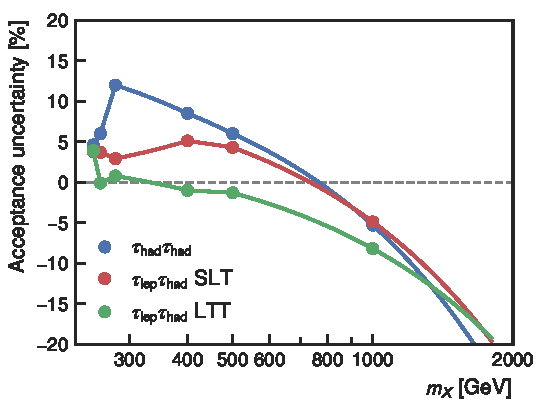
\includegraphics[scale=0.85]{uncertainties/resonant_ps_acc}

  \caption{Acceptance uncertainty on the BSM production of
    $gg \to X \to HH$ in the signal regions estimated from a
    comparison with an alternative parton shower program. A positive
    sign of the uncertainty indicates that the alternative
    configuration (\PYTHIA) predicts a larger \AccTimesEff than the
    nominal one (\HERWIG) and vice versa for negatively signed
    uncertainties. The lines indicate the linear inter- /
    extrapolation in \mX used to obtain the uncertainties for all
    other points of \mX considered in the analysis (hollow markers).}
  \label{fig:resonant_partonshower}
\end{figure}

Acceptance uncertainties from factorisation and renormalisation
scales, and PDF+\alphas are evaluated at generator-level for two mass
points with $\mX = \SI{500}{\GeV}$ and \SI{1000}{\GeV} after
approximating the selections applied in the analysis. The
uncertainties are found to be negligible and are therefore omitted.

An additional uncertainty is assigned in the \hadhad and \lephad LTT
channels to signal samples using fast simulation with
\textsc{ATLFAST-II}~\cite{SOFT-2010-01}. The efficiency of \tauhadvis
triggers is found to deviate between full and fast simulation, without
dedicated calibrations of \tauhadvis trigger efficiencies in fast
simulation being available. An uncertainty is estimated by comparing
the acceptance between full and fast simulation for a benchmark sample
at a mass of \SI{400}{\GeV}. The acceptance predicted using fast
simulation is \SI{6.5}{\percent} (\SI{3.6}{\percent}) larger than in
full simulation for the \hadhad (\lephad LTT) signal region for the
benchmark point. Distributions of kinematic and MVA input variables
are compared between fast and full simulation showing no significant
deviations in their shapes. Therefore, the difference in acceptance is
assigned as an additional normalisation uncertainty in the \hadhad and
\lephad LTT channel for all signal samples simulated using
\textsc{ATLFAST-II}~(i.e.\ $\mX \leq \SI{1000}{\GeV}$).

%%% Local Variables:
%%% mode: latex
%%% TeX-master: "../../phd_thesis"
%%% End:
